\documentclass[12pt]{report}

\usepackage[utf8]{inputenc}
\usepackage[T1]{fontenc}
\usepackage{listings}
\lstset{breaklines=true}
\usepackage[left=2cm,right=2cm,top=2cm,bottom=2cm]{geometry}
\usepackage[frenchb.ldf]{babel}
\usepackage{graphicx}
\usepackage[]{algorithm2e}


\title{Scanner Nmap Python}
\author {\bf Auteur\\\\
		Aurélien Bourillon\\
		Valentin Chaigneau\\
		Raphaël Dupin\\\\\\
		\bf Superviseur\\\\
		Nicolas Greneche\\\\\\\\}
\date{23/01/2017}

\begin{document}
\maketitle
\section*{Introduction}
	\paragraph{}
	Dans les entreprises, l'administration d'un parc informatique n'est pas une tâche facile. Les parcs sont de plus en plus grands et un administrateur réseau aura bien du mal à savoir quels services sont présents dans son parc. C'est pourquoi, dans le cadre de nos études, on nous a proposé de réaliser un scanner réseau permettant de connaître rapidement quels sont les services présents dans un parc informatique.	Le principe de ce scanner est assez simple. Il devra scanner un réseau donné pour enregistrer dans une base de données différentes informations que nous verrons plus tard. Ce scanner sera sous la forme d'un daemon pour faciliter l'automatisation. Ces résultats seront visibles via un SiteWeb qui permettra de générer un fichier de règles pour un firewall.
	\paragraph{}
	Ce rapport présentera les outils utilisés à savoir NMAP et l'API Python de NMAP. Nous exposerons ce que NMAP permet et pourquoi le choix du langage python est intéressant dans ce cas. Nous verrons ensuite l'installation et la configuration du daemon via les fichiers fournît. 
\tableofcontents
\part{Présentation du contexte}
	\chapter{NMAP}
		\paragraph{}
			NMAP ("Network Mapper") est un outil open source d'exploration réseau et d'audit de sécurité. Il permet l'analyse de plage réseau ou d'une machine précise. Grâce à des paquets IP bruts (raw packets), il peut déterminer de nombreuses informations concernant les services (port, nom du service, version...), mais aussi concernant la machine. En effet, NMAP permet de connaitre l'OS de la machine que nous analysons.
			\begin{lstlisting}[caption=Scan NMAP, captionpos=b]
# nmap -A -T4 81.194.43.80

Starting Nmap 7.40 ( https://nmap.org ) at 2017-01-25 13:17 CET
Nmap scan report for monitor.univ-paris13.fr (81.194.43.80)
Host is up (0.022s latency).
Not shown: 997 filtered ports
PORT      STATE  SERVICE VERSION
80/tcp    open   http    Apache httpd 2.2.8 ((Ubuntu))
|_http-server-header: Apache/2.2.8 (Ubuntu)
|_http-title: Did not follow redirect to /cacti/
443/tcp   closed https
20031/tcp open   unknown
Device type: general purpose
Running: Linux 2.6.X
OS CPE: cpe:/o:linux:linux_kernel:2.6
OS details: Linux 2.6.15 - 2.6.26 (likely embedded), Linux 2.6.29 (Gentoo)
Network Distance: 13 hops

OS and Service detection performed. Please report any incorrect results at https://nmap.org/submit/ .
Nmap done: 1 IP address (1 host up) scanned in 39.56 seconds
			\end{lstlisting}
			\paragraph{}
				Sur cet exemple nous pouvons voir que la machine analysée a trois services disponibles. HTTP est ouvert sur le port 80, HTTPS closed sur le port 443 et un autre service inconnu sur le port 20031. Il faut savoir que l'état "open" et "closed" sont assez courant mais ce ne sont pas les seuls. En effet, nmap peut voir un service en état "filtered" ou "unfiltered". Voici l'explication pour chacun de ces états :
			\begin{description}
			\item OPEN : Le service de la machine est en écoute sur ce port
			\item CLOSED : Aucun service en écoute sur ce port. Mais il peut s'ouvrir n'importe quand.
			\item FILTERED : Ici NMAP nous indique qu'un dispositif l'a empéché de déterminer si le service est ouvert ou fermé. Cela peut-être dû à un pare-feu par exemple.
			\item UNFILTERED : Ces ports sont particuliés, car ils répondent aux paquets test de NMAP, cependant NMAP ne peut pas déterminer s'ils sont ouverts ou fermés.
			\end{description}
			\paragraph{}
				En bref, NMAP offre de nombreuses possibilités qui peuvent répondre au projet que nous devons réaliser. Les explications précédentes ne sont qu'une petite partie de ce que peut faire NMAP. Il peut par exemple effectuer du reverse DNS, connaître le type de matériel de la machine ou même retrouver les adresses MAC.
	\chapter{Python}
		\section{Python en bref}
			\paragraph{}
				Python est un langage de programmation créé en 1991, mais baptisé seulement en 2001 (Python Software Foundation). Les informaticiens aiment penser que le nom de ce langage est une référence aux "Monty Python" dont Guido van Rossum était fan. Mais Concrètement qu'est-ce que Python ? Tout d'abord, il faut savoir que python est un langage facile (bien que son indentation reste un petit casse-tête) à apprendre, mais qui offre de nombreuses possibilités. Les programmes sont appelés script qui ont souvent une seule mission bien précise. Cependant, il est possible de réaliser des jeux vidéos, logiciels en tout genre voir même des progiciels (souvent utilisés par les professionnel, ce sont plusieurs logiciels fonctionnant ensemble).
			\paragraph{}
				Ce langage utilise un système de typage automatique. C'est-à-dire que lors de l'affectation d'une variable, Python va en déduire le typage (int, float, str...). Par exemple voici une suite de commande affectant une variable et dont on affichera le type :
				\begin{lstlisting}[caption=Affectation variable en Python, captionpos=b]
			>>> variable="Bonjour"
			>>> type(variable)
			<type 'str'>
			>>>
				\end{lstlisting}
			\paragraph{}
				Nous pouvons voir sur cet exemple que la variable est affectée à une chaîne de caractère. Python déduira alors son type automatiquement. Mais alors pourquoi utiliser Python dans notre projet ? Comme nous l'avons vu nous pouvons créer des scripts. Ce qui permettra d'automatiser le scan réseau plus facilement. Mais surtout Python à une API qui permet d'interagir avec NAP. C'est ce que nous allons voir maintenant.
		\section{l'API NMAP}
			\paragraph{}
				Dans cette partie nous allons exposer le fonctionnement et l'utilisation de l'API NMAP Python. Pour que cette API fonctionne, NMAP doit être installé sur la machine. Voici la démarche à suivre pour effectuer un scan sur la même machine que tout à l'heure mais en spécifiant une plage de port mais, en Python :
				\begin{lstlisting}[caption=Scan NMAP avec Python, captionpos=b]
>>> import nmap
>>> nm = nmap.PortScanner()
>>> nm.scan("81.194.43.80", "22-443", arguments='-sV')
{'nmap': {'scanstats': {'uphosts': '1', 'timestr': 'Wed Jan 25 14:12:35 2017', 'downhosts': '0', 'totalhosts': '1', 'elapsed': '15.91'}, 'scaninfo': {'tcp': {'services': '22-443', 'method': 'connect'}}, 'command_line': 'nmap -oX - -p 22-443 -sV 81.194.43.80'}, 'scan': {'81.194.43.80': {'status': {'state': 'up', 'reason': 'syn-ack'}, 'hostnames': [{'type': 'PTR', 'name': 'monitor.univ-paris13.fr'}], 'vendor': {}, 'addresses': {'ipv4': '81.194.43.80'}, 'tcp': {80: {'product': 'Apache httpd', 'state': 'open', 'version': '2.2.8', 'name': 'http', 'conf': '10', 'extrainfo': '(Ubuntu)', 'reason': 'syn-ack', 'cpe': 'cpe:/a:apache:http_server:2.2.8'}, 443: {'product': '', 'state': 'closed', 'version': '', 'name': 'https', 'conf': '3', 'extrainfo': '', 'reason': 'conn-refused', 'cpe': ''}}}}}
				\end{lstlisting}
			\paragraph{}
				Nous avons tout d'abord importé la libraire nmap, pour ensuite affecter une variable au PortScanner() de NMAP. Pour finir par lancer un scan en spécifiant une IP, une plage de port et des arguments NMAP. Mais finalement que fait l'API ? En fait, rien d'extraordinaire, si nous regardons les processus en cours lors de l'exécution de la commande :
				\begin{lstlisting}
$ ps aux | grep nmap
kungfury  3061 12.0  0.3  74708 31304 pts/1    S+   14:13   0:00 nmap -oX - 81.194.43.80 -p 22-443 -sV
				\end{lstlisting}
			\paragraph{}
				Nous pouvons remarquer que le script fait appel à NMAP avec l'option "-oX". Cette option permet de formater la sortie du scan au format XML. Une fois cette sortie récupérée, l'API n'a plus qu'à ranger les informations dans une structure que nous pourrons interroger par la suite. Elle est d'ailleurs affichée en sortie dans l'exemple de scan NMAP avec Python. Mais cette fonctionnalité ne sort pas seulement une structure. Nous le verrons plus en détail lorsque nous parlerons de notre solution finale, mais nous pouvons faire appel à différentes fonctions pour nous simplifier la vie. Voici un exemple qui permet de récupérer le nom d'un service sur une machine donnée.
				\begin{lstlisting}[caption=Récupération du nom d'un service, captionpos=b]
>>> nm.all_hosts()
['81.194.43.80']
>>> nm['81.194.43.80'].all_protocols()
['tcp']
>>> nm['81.194.43.80']['tcp'].keys()
[80, 443]
>>> nm['81.194.43.80']['tcp'][80]['name']
'http'
				\end{lstlisting}
		\section{L'API MYSQL}
			\paragraph{}
				Nous l'avons vu en introduction, les résultats trouvés par le script python seront stockés dans une base de données. Nous allons exposer ici comment dialoguer avec une base de données MYSQL en Python. Le paquet "python-connector" est nécessaire pour effectuer l'exemple suivant :
				\begin{lstlisting}[caption=Connexion à une base de données et insertion de données, captionpos=b]
>>> unnom="KungFury"
>>> import mysql.connector
>>> bdd = mysql.connector.connect(host='IP_BDD',user='nom_user',password='pass_user', database='nom_BDD')
>>> cursor = bdd.cursor()
>>> cursor.execute("""INSERT INTO exemple (nom) VALUES(%s)""", (unnom))
>>> bdd.commit()
				\end{lstlisting}
			\paragraph{}
				Dans cet exemple, nous nous sommes connectés à une base de données grâce à "mysql.connector". Une fois connecté nous récupérons un cursor qui permettra d'effectuer les requêtes SQL. Une fois la requête voulu mis en attente grâce au curseur, il suffit de commit avec l'objet "mysql.connector". Il est possible de faire plusieurs requêtes SQL avant de commit. Maintenant, voici la procédure à suivre pour récupérer des résultats (nous gardons les mêmes variables que précédemment) :
				\begin{lstlisting}[caption=Récupérationd de données, captionpos=b]
>>> query = 'SELECT ID FROM table WHERE nom = '+unnom
>>> cursor.execute(query)
>>> result = cursor.fetchone()
				\end{lstlisting}
			\paragraph{}
				Ici, nous avons récupéré un résultat grâce à la fonction "fetchone()". Il aurait été possible de récupérer plus de résultats grâce à la fonction "fetchall()". Nous aurions alors eu une liste de résultats.
	\chapter{Le projet}
		\paragraph{}
			Nous venons de voir les différents outils que nous allons utiliser pour réaliser le projet. Nous allons maintenant exposer le sujet de ce projet. Comme dit en introduction le but est de faire un scanner qui enregistrera les résultats dans une base de données. Nous avons pour consigne de récupérer les informations suivantes :
			\begin{itemize}
				\item Pour les machines :
					\begin{itemize}
						\item L'adresse IP
						\item Le FQDN (Fully Qualified Domain Name) : Position absolue d'un noeud dans une arborescence DNS
						\item La dernière fois que la machine a été vu
					\end{itemize}
				\item Pour les services :
					\begin{itemize}
						\item Le protocole
						\item Le port
						\item Le nom du service
						\item Son état
						\item La banner
						\item La version
						\item La dernière fois que le service a été vu
					\end{itemize}
			\end{itemize}
		\paragraph{}
			Un aspect important de l'administration d'un parc informatique est de savoir qui est présent sur le réseau et surtout à quel moment. C'est pourquoi nous devons récupérer la date où le scanner voit la machine ou le service. Si nous voyons un service ouvert à une telle date et que depuis ce service n'existe plus, nous pouvons nous poser des questions. Quoi qu'il en soit pour voir les machines de façon régulière le script doit être automatisé. C'est pourquoi nous allons en faire un daemon pour qu'il puisse agir en permanence. Uns fois ces tâches effectuée, les résultats seront visibles depuis une interface WEB. Ainsi, nous pourrons voir d'un coup d'oeil voir les machines et les services présents. Il y aura même la possibilité de générer un fichier de règles en fonctions des services que nous voulons ou non. Si par exemple, sur une machine, un service inconnu est en écoute sur le port 12345, l'administrateur réseau pourra sélectionner le fait qu'il ne désire pas le laisser passer. Le site générera un fichier de règles de pare-feu.
\part{Présentation et installation de la solution}
	\chapter{Prérequis}
		\paragraph{}
			Avant de se lancer dans l'installation de notre solution, plusieurs paquets doivent être présents sur la machine. Voici la liste des paquets nécessaires, ils sont en général présent dans les dépôts classiques d'une machine linux (Debian, Ubuntu...) :
			\begin{itemize}
				\item python-mysql.connector
				\item python-termcolor
				\item python-netaddr
				\item mysql-server
				\item nmap
			\end{itemize}
			\begin{lstlisting}[caption=Installation des paquets nécessaires, captionpos=b]
# apt-get update
# apt-get install python-mysql.connector python-netaddr python-termcolor mysql-server nmap
			\end{lstlisting}
		\paragraph{}
			Le script python utilise la version 2.7 de Python. Le daemon utilisera l'éxecutable "/usr/bin/python" pour executer le script.
	\chapter{Le script d'installation}
		\paragraph{}
			Pour l'installation de notre solution nous proposons un script qui installera toute la partie BDD (dont nous verrons la structure plus tard) et daemon. Nous avons au départ donc deux fichiers à savoir "install\_scanner.sh" et "jajscan.py" dont nous parlerons plus tard. Le script d'installation peut recevoir plusieurs arguments qui sont les suivants :
			\begin{description}
				\item install : Permet l'installation totale de la solution
				\item reinstall : Supprimera tous les fichiers de configurations, d'interaction avec la BDD, le daemon et les logs. Puis relancera l'installation.
				\item clearbdd : Permet de vider les tables créées à l'installation
				\item unistall : Supprimera la totalité de la solution et supprimera les tables dans la BDD.
			\end{description}
		\paragraph{}
			Pour installer la solution il faut néanmoins créer au préalable une Database. L'installateur se chargera de créer les tables. Il suffit pour lancer l'installation de faire comme suit :
			\begin{lstlisting}[caption=Installation, captionpos=b]
# chmod +x install_scanner.sh 
# ./install_scanner.sh install
Creation du dossier de log : /var/log/pythonnmap/
Creation du service...
Adresse de la BDD : 127.0.0.1
Nom de la base : Scanner
Nom utilisateur BDD : scanner_user
Mot de passe BDD : 
Reseau a analyser [0.0.0.0/24] : 192.168.10.0/24
Port a analyser [Port_debut-Port_fin / all] : all
NOTE : En vitesse fast l analyse est moins precise !
Vitesse d analyse [fast/slow] : slow
Voulez-vous utiliser un Time Out ? [y/n]y
Utiliser le Time Out automatique (Se basera sur la premiere machine scanee)? [y/n]y
Voulez-vous recevoir les resultats du scan par mail (SMTP uniquement)? [y/n]n
Creation du fichier de configuration...
Creation des script SQL...
Renseignez un utilisateur disposant des droits CREATE/ALTER sur la table  Scanner
Nom utilisateur : root
Mot de passe :
			\end{lstlisting}
		\paragraph{}
			Durant l'installation, un certain nombre de questions sont posés afin de bien configurer le daemon. Suite à cette installation plusieurs dossiers et fichiers sont créés :
			\begin{figure}[ht]
				\begin{center}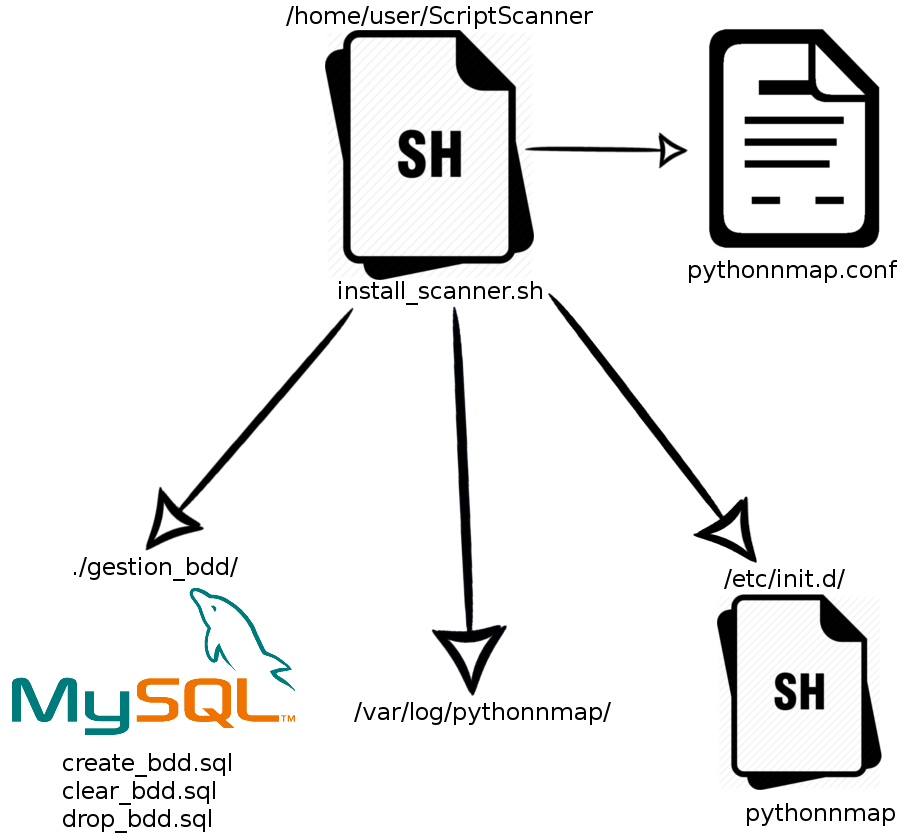
\includegraphics[height=250pt,keepaspectratio]{/home/valentin/Python_scan/Rapport/IMG/Install.png}
				\caption{\label{create_file} Fichiers et dossiers créés suite à l'installation}\end{center}
			\end{figure}
		\paragraph{}
			Comme nous pouvons le voir, l'installation a créé :
			\begin{itemize}
				\item Les fichiers SQL permettant au script d'installation d'interragir avec la BDD
				\item Le dossier où se trouveront les logs du daemon
				\item Le daemon "pythonnmap"
				\item Le fichier de configuration du daemon
			\end{itemize}
		\paragraph{}
			Ce fichier de configuration sera lu par le daemon pour lire les différents paramètres du scan. Ainsi, nous ne sommes pas obligés de réinstaller toute la solution si nous décidons de changer la cible du scan.
			\begin{lstlisting}[caption=Exemple fichier de configuration, captionpos=b]
############# CONFIGURATION SCANNER PYTHON NMAP #############
BDDAddr = 127.0.0.1
BDDName = Scanner
BDDUser = scanner_user
BDDPass = user@pass
Reseau = 192.168.10.0/24
## Format : PortDebut-PortFin ou mettre all pour scanner tout les ports
Port = all
## Format : slow ou fast (le mode fast est moins precis)
Speed = slow
################ GESTION TIMEOUT ################
UseTimeOut = y
UseAutomaticTimeOut = y
SetTimeOut = 00:00:00
########### CONFIGURATION MAIL SCANNER PYTHON NMAP ###########
## Mettre y pour activer l envoie de mail
Envoimail = n
AddrSend = 
Passmail = 
##Adresse destination format : mail1, mail2, mail3...
AddrDest = 
AddrSMTP = 
PortSMTP =

			\end{lstlisting}
		\paragraph{}
			Le daemon offre la possibilité d'envoyer les résultats par mail et de gérer un time out (nous le verrons en détail plus tard). Dans ce fichier il faudra renseigner les différents paramètres de serveur mail (seulement SMTP). Le paramètre "speed" permet de spécifier si le daemon utilisera les threads NMAP ou non (mode fast pour les utiliser). En sachant que ce mode est moins précis et peut ne pas remonter les résultats demandé. De plus, il est possible de spécifier une time out. Soit en le fixant, soit en utilisant la mode "automatique". Celui-ci se basera sur la première machine du scan et ajoutera une minute (marge d'erreur).
	\chapter{La base de données}
		\paragraph{}
			Nous l'avons vu durant l'installation, il est nécessaire de créer une base de données. Le script d'installation va lui créer les tables qui permettront de stocker les informations recueilli par le scanner. Il y aura deux tables à savoir une table "machines" et une table "services". Elles seront configurées comme suit :\\
			\begin{table}[h]
			\centering
			\begin{tabular}{|c|c|}
				\hline
					Nom & Type \\
				\hline
				\hline
					mid & int \\
				\hline
					fqdn & text \\
				\hline
					ip & text \\
				\hline
					last\_view & datetime\\
				\hline
			\end{tabular}
			\caption{\label{machines_bdd} Table Machines}
			\end{table}
			\begin{table}[h]
			\centering
			\begin{tabular}{|c|c|}
				\hline
					Nom & Type \\
				\hline
				\hline
					sid & int \\
				\hline
					mid & int \\
				\hline
					proto & text \\
				\hline
					port & int \\
				\hline
					nom\_service & text \\
				\hline
					sate & text \\
				\hline
					banner & text \\
				\hline
					version & text \\
				\hline
					last\_view & datetime \\
				\hline
					manage & int \\
				\hline
			\end{tabular}
			\caption{\label{services_bdd} Table Services}
			\end{table}
		\paragraph{}
			Ces tables sont liées par le "mid" qui est l'ID de la machine. Cette clé étrangère présente dans la table "services" permet de faire rapidement le lien avec la machine associée. La colonne "manage" est présente pour savoir si le service a été pris en compte par l'utilisateur via l'interface WEB.
	\chapter{Le daemon}
		\paragraph{}
			Nous avons vu l'installation et la base de données qui en découlent. Maintenant, nous allons voir le daemon. Dans cette partie nous ne parlerons pas du script Python, mais de comment il est appelé et géré. Lors de la création du daemon, le script a pris en compte les options de l'utilisateur ainsi que le dossier courant. C'est-à-dire qu'il a créé un daemon sur mesure en fonction d'où se trouve le script d'installation et le scanner Python. Le scanner sera appelé avec un argument qui sera le fichier de configuration qui se trouve aussi dans le dossier du script d'installation. Le daemon pourra ainsi être lancé grâce à la commande :
			\begin{lstlisting}
			# service pythonnmap start
			\end{lstlisting}
		\paragraph{}
			Le script Python tournera alors comme un service. Etant donné qu'il possède une boucle infini celui-ci continuera sont éxecution jusqu'à l'arrêt du service ou de la machine. Lorsque l'administrateur stop le service, celui-ci envoie le signal "KeyboardInterrupt" au script.
\part{Le script Python}
	\chapter{D'un point de vue général}
		\paragraph{}
			Dans cette partie nous allons le fonctionnement général du script. Nous allons voir son file d'éxecution sans vraiment détailler les fonctions qu'il parcourt. Le détail de ces fonctions se fera dans la partie suivante.\\
			Comme nous l'avons vu dans le chapitre sur le daemon, celui-ci fait appel au script avec un argument. Cet argument sert à localiser le fichier de configuration. S'il n'est pas renseigné, le script considérera qu'il se trouve dans le dossier courant sous le nom de "pythonnmap.conf" :
			\begin{lstlisting}[caption=Récupération path fichier configuration, captionpos=b]
if len(sys.argv) == 2:
    path_conf=sys.argv[1]
else:
    path_conf="pythonnmap.conf"
			\end{lstlisting}
		\paragraph{}
			Une fois le path récupéré le script commence sa boucle infini. Il va alors commencer son scan en fonction des paramètres présents dans le fichier de configuration. Quelle que soit la plage IP renseignée, le scanner va faire les machines une par une. Cela apporte une meilleure visibilité lors d'un scan sur un grand parc. Si dans le fichier de configuration l'administrateur a spécifié "192.168.1.0/24", le script déduira les IP possible. De même pour une plage IP de la forme "192.168.1.24-52".
		\paragraph{}
			Pour chaque adresse IP, un scan sera effectué en fonction des ports renseignés et du mode voulu (fast ou slow). Une fois les informations récupérées, le programme va stocker ces informations dans deux structures. Une structure "Host" et une structure "Service" qui correspondent aux tables présentes dans la base de données. La structure "Host" disposera d'un tableau de "Service" pour qu'une machine soit liée à tous ses services. Si jamais le time out est atteint, le programme va alors lancer un nouveau scan avec des options sensées rendre le scan plus rapide. Il sera normalement moins complet mais aboutira à quelques résultats. Si encore une fois ce n'est pas le cas, le programme passera à la machine suivante.
		\paragraph{}
			Le stockage des machines étant terminé, le programme va maintenant insérer les informations dans la base de données. Plusieurs cas sont alors possibles :
			\begin{itemize}
				\item La machine n'est pas connu dans la BDD : Le script fera une insertion de toutes les informations
				\item La machine est connu dans la BDD : Le script fera seulement un update de la date (colonne "last\_view")
				\item Le service n'est pas connu dans a BDD : Le script fera une insertion de toutes les informations
				\item Le service est connu dans la BDD : Le script va alors analyser son nom, son état, sa banner et sa version en fonction de la BDD. Il fera un update des informations qui auront changées. Il fera aussi un update de la date (colonne "last\_view")
			\end{itemize}
		\paragraph{}
			Une fois l'insertion en BDD terminée, le script va soit terminer et recommencer, ou alors envoyer les résultats par mail avant de recommencer. Si c'est le cas, le script va remplir un fichier ".csv" (fichier tableur) qu'il mettra en pièce jointe du mail qui sera envoyé. L'envoi du mail se basera aussi sur les informations renseignées dans le fichier de configuration.
	\chapter{Algorithme principal}
		\paragraph{}
			Dans cette partie nous allons voir l'algorithme principal du programme.
			\begin{algorithm}
			 \eIf{longueur\_argument > 1}{
			 	path\_conf = argument[2]
			 }{
			 	path\_conf = "pythonnmap.conf"
			 }
			 \While{true}{
			 	\For {ip\_debut to ip\_fin}{
			 		start\_thread\_scanner()\\
			 		\If{ReadConf("WantTimeOut") = 'y'}{
			 			start\_thread\_timeout()
			 		}
			 		wait\_thread\_scanner()\\
			 		\eIf{result\_scanner = 'None'}{
			 			start\_thread\_scanner\_simple()\\
			 			\If{ReadConf("WantTimeOut") = 'y'}{
					 			start\_thread\_timeout()
					 	}
					 	\eIf{result\_scanner = 'None'}{
					 		print(Scan impossible)\\
					 	}{
					 		start\_analyze\_and\_insertion\_bdd()
					 	}
			 		}{
			 			start\_analyze\_and\_insertion\_bdd()
			 		}
			 	}
			 	\If{ReadConf("SendMail") = 'y'}{
			 		send\_mail()
			 	}
			 }
			 \caption{Main algortithm jajscan.py}
			\end{algorithm}
	\chapter{Structures}
		\section{class Host}
			{\setlength{\parindent}{0cm}
			$Propri\acute{e}t\acute{e} :$
			}
			\begin{description}
				\item ip : IP de la machine
				\item serv : Tableau de structure Service
				\item fqdn : FQDN de la machine
				\item date : Date où la machine a été vu
			\end{description}
			$Description :$ Cette structure permet de paramétrer une machine. Elle correspond en tout point à la base de données sauf qu'elle est liée au service via un tableau de la class "Service".
		\section{class Service}
			{\setlength{\parindent}{0cm}
			$Propri\acute{e}t\acute{e} :$
			}
			\begin{description}
				\item port : Port du service
				\item version : Version du service
				\item nomservice : Nom du service
				\item state : Etat du service
				\item banner : Bannière du service
				\item proto : Protocole du service
			\end{description}
			$Description :$ Cette structure permet de paramètrer un service. C'est cette class qui est "liée" à la class "Host". Elle correspond en tout point à la base de données.
		\section{class TimeOutThread}
			{\setlength{\parindent}{0cm}
			$Propri\acute{e}t\acute{e} :$
			}
			\begin{description}
				\item run : Main du thread
				\item stop : Permet de stopper le thread
			\end{description}
			$Description :$ Nous retrouvons ici le thread de time out. Celui-ci se basera sur la configuration présente dans le "pythonnmap.conf".
		\section{class ScannerThread}
			{\setlength{\parindent}{0cm}
			$Propri\acute{e}t\acute{e} :$
			}
			\begin{description}
				\item run : Main du thread
			\end{description}
			$Description :$ Ce thread permet de lancer le scan NMAP. Ce thread est attendu dans le main principal. S'il prend trop de temps il sera killé par le thread de time out.
	\chapter{Fonctions}
		\section{analyze()}
			{\setlength{\parindent}{0cm}
			$Nom :$ analyze\\\\
			}
			$Arguments :$
			\begin{description}
				\item nm : Objet NMAP\\
			\end{description}
			$Description : $ Cette fonction permet de trier les informations stockées dans l'objet NMAP. Elle remplira les structures "Host" et "Service" puis appellera la fonction "start\_insert()"
		\section{check\_element\_service()}
			{\setlength{\parindent}{0cm}
			$Nom :$ check\_element\_service\\\\
			}
			$Arguments :$
			\begin{description}
				\item check : Nom de la colonne de la table "services" à vérifier
				\item newval : Valeur à comparer avec la colonne de la table "services"
				\item port : numero du port associé au service
				\item mid : identifiant de la machine
				\item cursor : Curseur lié à la BDD\\
			\end{description}
			$Description : $ Cette fonction permet de vérifier les informations stockées dans la BDD. La variable check aura par exemple comme affectation "nom\_service", "banner", "state" ou "version". Par la suite elle va comparer la nouvelle valeur ("newval") avec ce qu'y est présent dans la BDD.  Elle prendra soin de comparer ces valeurs en fonctions d'une machine et d'un port.
		\section{connect\_bdd()}
			{\setlength{\parindent}{0cm}
			$Nom :$ connect\_bdd\\\\
			}
			$Arguments :$\\\\
			$Description : $ Cette fonction permet la connexion avec la BDD en fonction des informations stockées dans le fichier de configuration "pythonnmap.conf". Elle retournera un objet "mysql.connector" qui permettra le dialogue avec la BDD ainsi que la récupération du cursor pour les requêtes SQL.
		\section{datestr()}
			{\setlength{\parindent}{0cm}
			$Nom :$ datestr\\\\
			}
			$Arguments :$
			\begin{description}
				\item tmp\_time : Date à convertir\\
			\end{description}
			$Description : $ Cette fonction permet de convertir un objet Python date en String au format HH:MM:SS.
		\section{define\_ip\_addr()}
			{\setlength{\parindent}{0cm}
			$Nom :$ define\_ip\_addr\\\\
			}
			$Argument :$
			\begin{description}
				\item rangeip : Plage IP\\
			\end{description}
			$Description : $ Cette fonction permet de déduire les IP possible dans une plage IP. Cette fonction attend en paramètre soit la forme "X.X.X.0/XX" ou la forme "X.X.X.X-X". Ainsi, la fonction retournera une liste d'IP pour pouvoir scanner les IP une par une.
		\section{get\_sec()}
			{\setlength{\parindent}{0cm}
			$Nom :$ get\_sec\\\\
			}
			$Argument :$
			\begin{description}
				\item time\_str : Temps à convertir (au format 00:00:00)\\
			\end{description}
			$Description :$ Cette fonction permet de convertir un temps au format 00:00:00. Elle retournera ce temps en secondes.
		\section{get\_time()}
			{\setlength{\parindent}{0cm}
			$Nom :$ get\_time\\\\
			}
			$Argument :$
			\begin{description}
				\item seconds : Secondes à convertir
			\end{description}
			$Description :$ Cette fonction permet de convertir des secondes (sous forme d'entier) en temps au format 00:00:00.
		\section{insertmachine()}
			{\setlength{\parindent}{0cm}
			$Nom :$ insertmachine\\\\
			}
			$Arguments :$
			\begin{description}
				\item machine : Objet "Host"
				\item cursor : Curseur lié à la BDD\\
			\end{description}
			$Description : $ Cette fonction permet d'insérer une machine dans la BDD. Grâce à l'objet "Host", passé en paramètre, la fonction pourra récupérer facilement les informations liées à une machine. A savoir son IP, son FQDN et la date où elle a été vue.
		\section{insertport()}
			{\setlength{\parindent}{0cm}
			$Nom :$ insertport\\\\
			}
			$Arguments :$
			\begin{description}
				\item mid : Identifiant de la machine
				\item listport : Liste d'objet "Service"
				\item date : Date où les services ont été vu
				\item cursor : Curseur lié à la BDD\\
			\end{description}
			$Description : $ Cette fonction permet d'insérer les services lié à une machine dans la BDD. Contrairement à son nom, la fonction attend une liste de la structure "Service" et non seulement une liste de port.
		\section{interruptprogram()}
			{\setlength{\parindent}{0cm}
			$Nom :$ interruptprogram\\\\
			}
			$Arguments :$
			\begin{description}
				\item *args : Argument de l'interruption\\
			\end{description}
			$Description : $ Cette fonction est appelée lorsque le script reçoit une interruption clavier. Elle stoppera le programme et coupera la connexion avec la BDD si jamais elle est toujours ouverte.
		\section{readconf()}
			{\setlength{\parindent}{0cm}
			$Nom :$ readconf\\\\
			}
			$Arguments :$
			\begin{description}
				\item param : Configuration recherchée\\
			\end{description}
			$Description : $ Cette fonction permet de retourner la valeur d'un argument provenant du fichier de configuration. Par exemple grâce à l'appel "readconf("Reseau")", nous obtiendrons la plage IP que l'administrateur a spécifié dans le "pythonnmap.conf".
		\section{result\_to\_text\_file()}
			{\setlength{\parindent}{0cm}
			$Nom :$ result\_to\_text\_file\\\\
			}
			$Arguments :$
			\begin{description}
				\item temptotal : Temps total du scan
				\item cursor : Curseur lié à la BDD\\
			\end{description}
			$Description : $ Cette fonction n'est \textbf{plus utilisée} dans la version actuelle du script. Elle permet de mettre les résultats présents dans la BDD sous forme de fichier texte. Elle reste présente si jamais il est préférable, dans l'avenir, de recevoir les résultats par mail sous forme de fichier texte.
		\section{result\_to\_csv\_file()}
			{\setlength{\parindent}{0cm}
			$Nom :$ result\_to\_csv\_file\\\\
			}
			$Arguments :$
			\begin{description}
				\item temptotal : Temps total du scan
				\item cursor : Curseur lié à la BDD\\
			\end{description}
			$Description : $ Cette fonction permets de mettre les résultats présent dans la BDD sous forme de fichier "csv". Lorsque l'utilisateur demande de recevoir les résultats par mail, c'est cette fonction qui générera le fichier mit en pièce jointe du mail.
		\section{returnmid()}
			{\setlength{\parindent}{0cm}
			$Nom :$ returnmid\\\\
			}
			$Arguments :$
			\begin{description}
				\item ip : IP de la machine
				\item cursor : Curseur lié à la BDD\\
			\end{description}
			$Description : $ Cette fonction permet de retourner le "mid" d'une machine en fonction de son IP. Elle ira chercher cette information dans la BDD.
		\section{returnportmid()}
			{\setlength{\parindent}{0cm}
			$Nom :$ returnportmid\\\\
			}
			$Arguments :$
			\begin{description}
				\item mid : Identifiant de la machine
				\item cursor : Curseur lié à la BDD\\
			\end{description}
			$Description : $ Cette fonction permet de retourner une liste de port associé à une machine en fonction de son "mid". Elle ira chercher cette information dans la BDD.
		\section{returnsid()}
			{\setlength{\parindent}{0cm}
			$Nom :$ returnsid\\\\
			}
			$Arguments :$
			\begin{description}
				\item port : Port du service
				\item cursor : Curseur lié à la BDD\\
			\end{description}
			$Description : $ Cette fonction permet de retourner le "sid" d'un service en fonction de son port. Elle ira chercher cette information dans la BDD.
		\section{start\_insert()}
			{\setlength{\parindent}{0cm}
			$Nom :$ start\_insert\\\\
			}
			$Arguments :$
			\begin{description}
				\item listehost : Liste d'objet "Host"\\
			\end{description}
			$Description : $ Cette fonction permet de lancer l'insertion des informations en BDD. Grâce à une liste d'objet "Host", elle fera appel aux fonctions "insertmachine" et "insertport" qui seront déduire les informations stockées dans la liste. Par la suite elle fera un commit des requêtes fais dans les deux fonctions. 
		\section{send\_result\_mail()}
			{\setlength{\parindent}{0cm}
			$Nom :$ send\_result\_mail\\\\
			}
			$Arguments :$
			\begin{description}
				\item reseau : Réseau scannée par le scanner\\
			\end{description}
			$Description : $ Cette fonction permet l'envoi des résultats du scanner par mail. Elle fera d'abord appel à la fonction "result\_to\_csv\_file" pour ensuite joindre le fichier généré en pièce jointe. Le programme enverra en fonction des paramètres renseignés dans le fichier "pythonnmap.conf" et inscrira dans l'objet du mail "Resultat script" et dans le corps "Je suis le script python et voici les resultats pour le reseau ...".
		\section{start\_scan()}
			{\setlength{\parindent}{0cm}
			$Nom :$ start\_scan\\\\
			}
			$Arguments :$
			\begin{description}
				\item ip : IP à scanner
				\item port : Plage de port à scanner
				\item mode : Vitesse du scan "fast" ou "slow"\\
			\end{description}
			$Description : $ Cette fonction permet de lancer le scan NMAP. Elle prendra en compte la vitesse choisi par l'utilisateur. Si la vitesse est "fast", le programme utilisera les threads NAMP. Dans le cas contraire il fera un scan normal utilisant les paramètres "-sV -f --script banner".
		\section{writelog()}
			{\setlength{\parindent}{0cm}
			$Nom :$ writelog\\\\
			}
			$Arguments :$
			\begin{description}
				\item chaine : Chaine de caractère à écrire dans les logs\\
			\end{description}
			$Description : $ Cette fonction permet d'écrire dans les logs. Dans tout le programme, sont présent des appels à cette fonction. Il suffit juste de renseigner l'erreur en paramètre et celle-ci sera renseignée dans les logs avec la date d'écriture du log.
\part{L'interface WEB}
	\paragraph{}
		Nous l'avons vu dans la présentation du projet, une interface web permet de visualiser les machines scannées. Cette interface permet aussi de générer un fichier de règles pour un pare-feu.
		\begin{figure}[ht]
			\begin{center}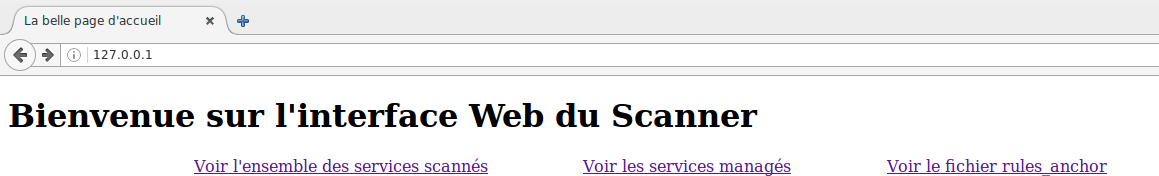
\includegraphics[width=500pt,keepaspectratio]{/home/valentin/Python_scan/Rapport/IMG/accueil.png}
			\caption{\label{accueil} Accueil de l'interface WEB}\end{center}
		\end{figure}
	\paragraph{}
		Depuis l'accueil nous pouvons choisir ce que nous voulons faire. Nous pouvons par exemple aller dans "Voir l'ensemble des services scannés" :
		\begin{figure}[ht]
			\begin{center}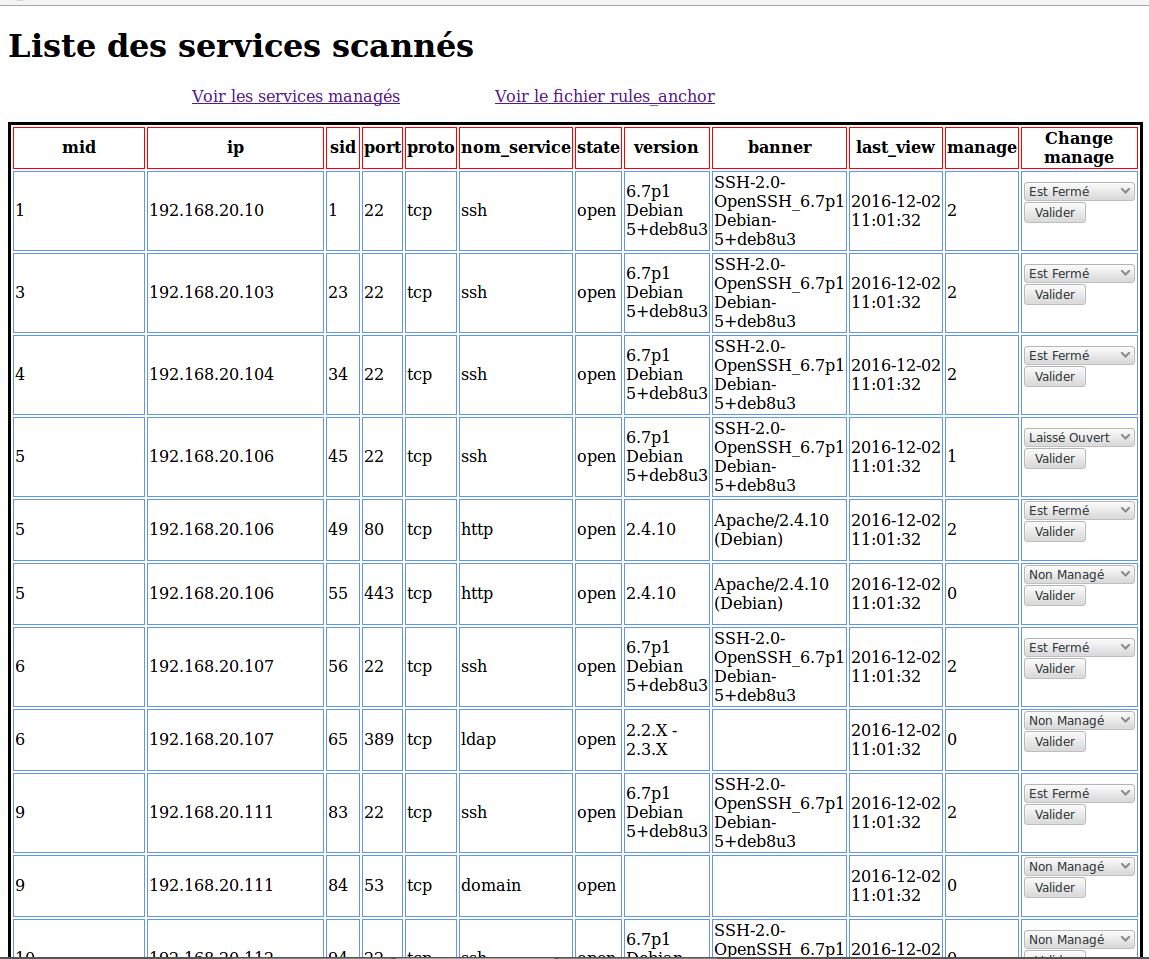
\includegraphics[width=400pt,keepaspectratio]{/home/valentin/Python_scan/Rapport/IMG/liste_service.png}
			\caption{\label{list_service} Liste services scannés}\end{center}
		\end{figure}
	\paragraph{}
		Via cette interface, nous pouvons visualiser l'ensemble des machines et des services scannés. C'est ici aussi que nous pouvons choisir de changer le traitement du service. Par défaut, les services sont dans l'état "Non Managé". L'administrateur pourra alors choisir de changer pour fermer le service ou le laisser ouvert via les état "Est fermé" et "Laissé Ouvert".
	\paragraph{}
		En validant, l'administrateur ajoutera la règle dans le fichier de règles. Une fois le service managé et validé, nous pouvons le retrouver sur cette interface :
		\begin{figure}[ht]
			\begin{center}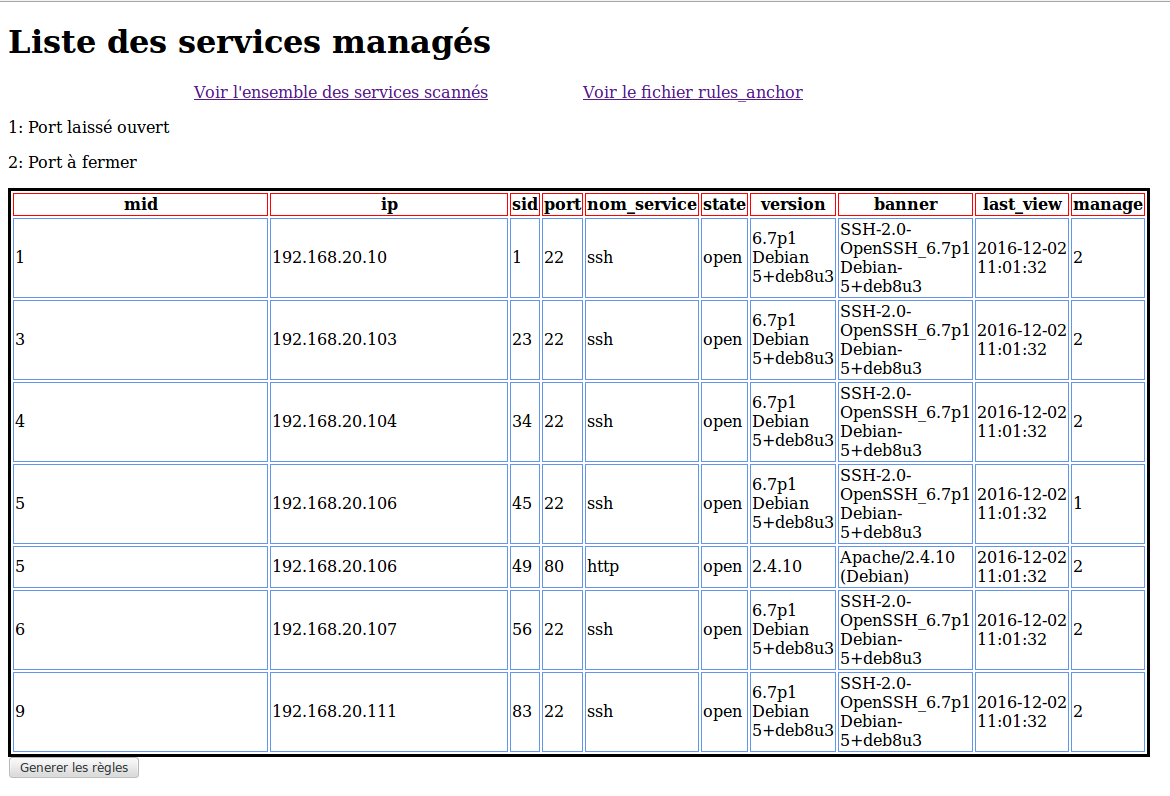
\includegraphics[width=400pt,keepaspectratio]{/home/valentin/Python_scan/Rapport/IMG/service_manages.png}
			\caption{\label{service_manage} Liste services managés}\end{center}
		\end{figure}
	\paragraph{}
		Il suffira à l'administrateur de cliquer sur le bouton "Générer les règles", en bas à gauche, pour que le fichier "rules\_anchor.txt" soit totalement regénèré. C'est-à-dire que toutes les règles seront supprimées puis remisent dans le fichier (utile si l'administrateur veut réouvrir l'accès à un service qu'il a fermé). Ce fichier contient alors les règles de pare-feu adapté à ce que l'administrateur a choisi de manager.
		\begin{figure}[ht]
			\begin{center}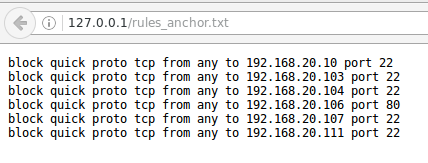
\includegraphics[width=300pt,keepaspectratio]{/home/valentin/Python_scan/Rapport/IMG/rules.png}
			\caption{\label{rules} Exemple fichier règles pare-feu}\end{center}
		\end{figure}
\end{document}